\section{Auditor Extension} \label{sec:auditor}
Until now we have not verified whether a certificate chain is logged as promised
by any issued SCT.  Our base design can be extended to follow-up on inclusion
statuses rather than opting for cross-logging.  In terms of
the number of necessary changes, this extension is more significant when
compared to Section~\ref{sec:log}.  However, it does not require any log
modifications, and it entails additional ecosystem value by providing a
well-audited view of the CT landscape which is captured by the Tor consensus.
It is possible to detect internal inconsistency attacks within the Tor
network and omission attacks.  Trust in some logs is also shifted towards CT
auditors.

\subsection{Design Sketch}
Figure~\ref{fig:auditor} provides an overview of the extended design.  Tor
Browser submits presented SFOs probabilistically to CTRs that are selected at
random, and CTRs mix the submitted SFOs before any auditing takes place.  Here,
auditing refers to inclusion verification rather than cross-logging.  The moment
before an SFO is audited, it is shared with a watchdog-CTR that is reused during
an entire auditing instance.  Unless an SFO is acknowledged as verified within a
timely manner by the log-challenging CTR, it is submitted by the watchdog to a
CT auditor.  Phase~1 remains unchanged, phase~2 needs minor changes, and phase~3
major changes.  Flushing statistics are also required in the extra-info
document, as well as additional parameters in the Tor consensus.  A final
prerequisite is that there are CT auditors available.

\begin{figure*}
    \centering
    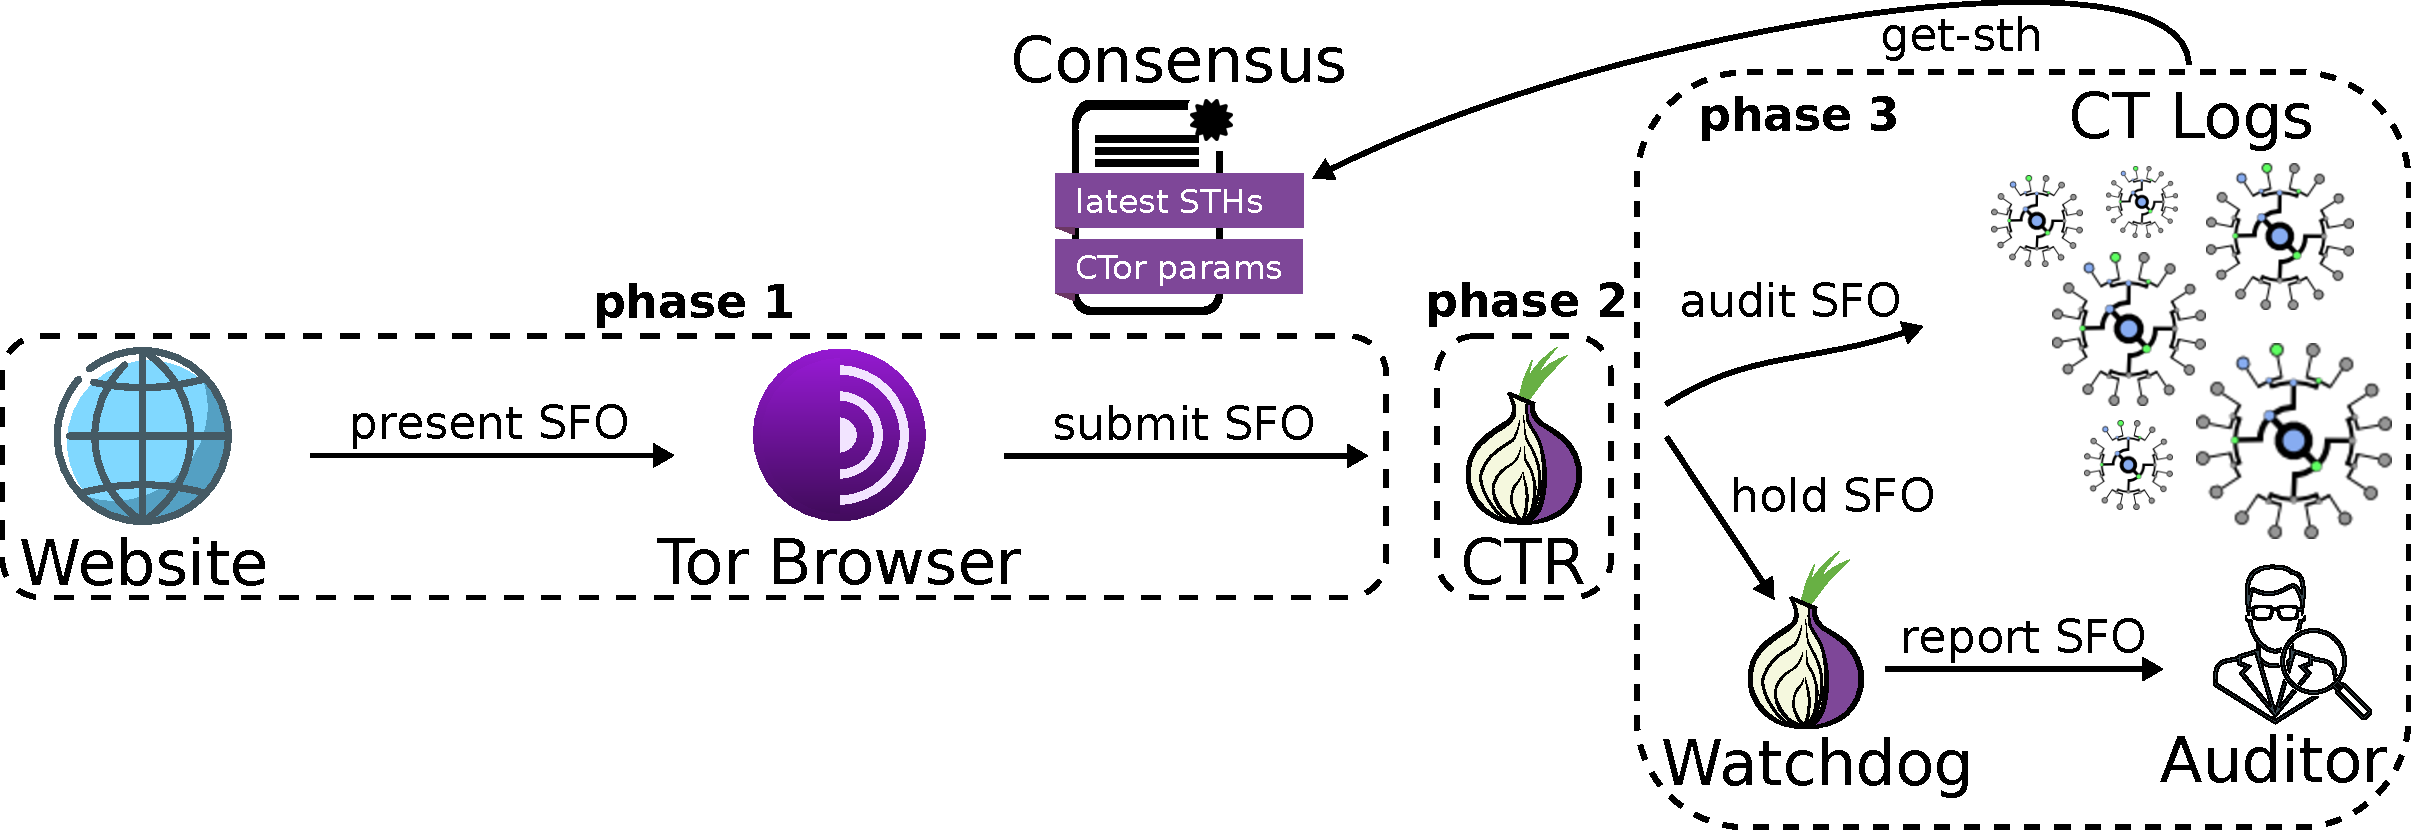
\includegraphics[width=0.85\textwidth]{img/design-auditor}
    \caption{todo}
	\label{fig:auditor}
\end{figure*}

\subsubsection{Tor Consensus}
Tor's consensus should capture a fixed view of the CT landscape by publishing
STHs from all recognized logs.  A log is recognized if a majority of directory
authorities proposed a \texttt{ct-log-info} item, which contains a log's ID,
public key, base URL, MMD, and most recent STH.  Note that each directory
authority proposes its own STH, and agrees to use the most recent STH as
determined by timestamp.  Since CTRs verify inclusion statuses of SCTs
that Tor Browser accepts, the CT logs recognized by Tor Browser must be in
the consensus.

Tor's directory authorities also majority-vote on \texttt{ct-auditor} items,
which pin base URLs and public keys of CT auditors that watchdogs contact in
case that any log misbehavior is suspected.  A watchdog triggers if the
\texttt{ct-watchdog-timeout} elapses without acknowledgment.  The following
auditor submission times-out if \texttt{ct-auditor-timeout} elapses.  These
items are determined similar to the \texttt{ct-query-timeout} in
Section~\ref{sec:base:consensus:params}.

\subsubsection{Phase~2: Storage}
A CTR cannot verify an SCT from an unrecognized log.
Step~\ref{enm:ctr-api:unrecognized} should therefore be updated so that
unrecognized SCTs are discarded, stopping if no SCTs remain in the resulting
SFO.  If an SFO is neither cached nor pending, sample an SCT and note down the
outcome and a corresponding \texttt{audit\_after} timestamp using
Equation~\ref{eq:audit-after}.  The combination of SFO, sampled SCT outcome, and
\texttt{audit\_after} timestamp is stored in the pending buffer.

\subsubsection{Phase~3: Auditing}

%
% Phase 3---Auditing
% - Major differences
%   --> establish connection to a random watchdog (add step 1.75)
%   --> step 3 needs a complete rewrite from (b) and forward
%
% Step 3
% b) continue if SFO.audit_after > STH.timestamp
% c) Submit SFO to watchdog
% d) Use ct-query-timeout and STH.treesize to set a timer and challenge the log
% to prove inclusion.
% - On valid proof: send ACK to watchdog, cache SFO, discard SFO from buffer
% - On any other outcome: discard SFO and break the loop
%
% Behavior of watchdog:
% - Listen for submissions on a dedicated endpoint
% - If a submitted SFO is not ACKed within the watchdog timeout
%   --> submit it to an announced auditor.
%   --> resubmit later on if auditor(s) unavailable; not entirely sure which
%   details we should go with here for the resubmission(s)
%

\subsubsection{Auditor}
% Readd what we had before

\subsection{Security Sketch}

%
% Extra-info document
% - Need flushing statistics
%

%
% MISC notes
% - Network-wide flush, detectable but hard to attribute
% - Requires new reliable auditor software
% - Bit more bandwidth due to watchdog.  The overhead, when compared to log a
% log extension, is sending an SCT hash and receiving a proof (2-3KiB).
%
